\documentclass[10pt]{article}
\usepackage[margin=.67in]{geometry}
\usepackage{amsmath,amssymb,graphicx,booktabs,hyperref,xcolor}
\hypersetup{colorlinks=true,urlcolor=blue}
\setlength{\parindent}{0pt}\setlength{\parskip}{6pt}
\newcommand{\scope}{\textcolor{gray}{\footnotesize Producer evidence; unsigned/unverified.}}
\begin{document}
{\Large\bf Fixed templates, shared columns, and the next selector}\par
Curve25519 index-calculus research \hfill 24 November 2026

\textbf{Result and scope.} A conditional finite-incidence argument excludes
constant-shape, fresh-query, equality-only tagged-row recovery below
square-root-order queries. It allows \emph{all} decompositions per query.
This is a statement about that model, with explicit original-map hypotheses.
It is not a lower bound for all coordinate methods or all adaptive bases.
The written argument is in \texttt{DERIVATION.md}; no new native run is used.

\textbf{Original map.} Assume the rational raw group has order $8\ell$,
eight rational points killed by $8$, and cyclic image of odd prime order
$\ell$. Preserve unique-rational-branch admission before zero/torsion
filtering. For a raw point $(x,y)$ and admitted $z=(u,v)$,
\[
 x=\frac{A(\epsilon-u)}{2u},\qquad
 u=\frac{\epsilon A}{2x+A},\qquad v^2=(u^2-1)/2,\quad \epsilon=\pm1.
\]
With nonzero $A,u$ and odd characteristic, at most four encodings occur per
raw point. The eight raw preimages give at most $32$ encodings per image.
Negating raw points preserves $x$ and the available signed encodings, so the
physical column $\{P,-P\}$ has the same bound, not twice it.

\textbf{Fixed roles imply bounded incidence.} Fix unit relative parameters
$\alpha_1,\ldots,\alpha_m$ before fresh queries. A witness uses
$z_i=\sigma\alpha_i$. Fixing a column, its role and one encoding fixes
$\sigma$. There are at most $2^m$ signed raw tuples at that multiplier, each
with one target sum. If $S(T)$ contains every column in any valid witness,
\[
 d(P):=\#\{T\ne0:P\in S(T)\}\le C_m:=32m2^m,\qquad C_2=256.
\]
Raw distinctness and base-range guards only reduce this upper count.
All cofactor sectors are already included.

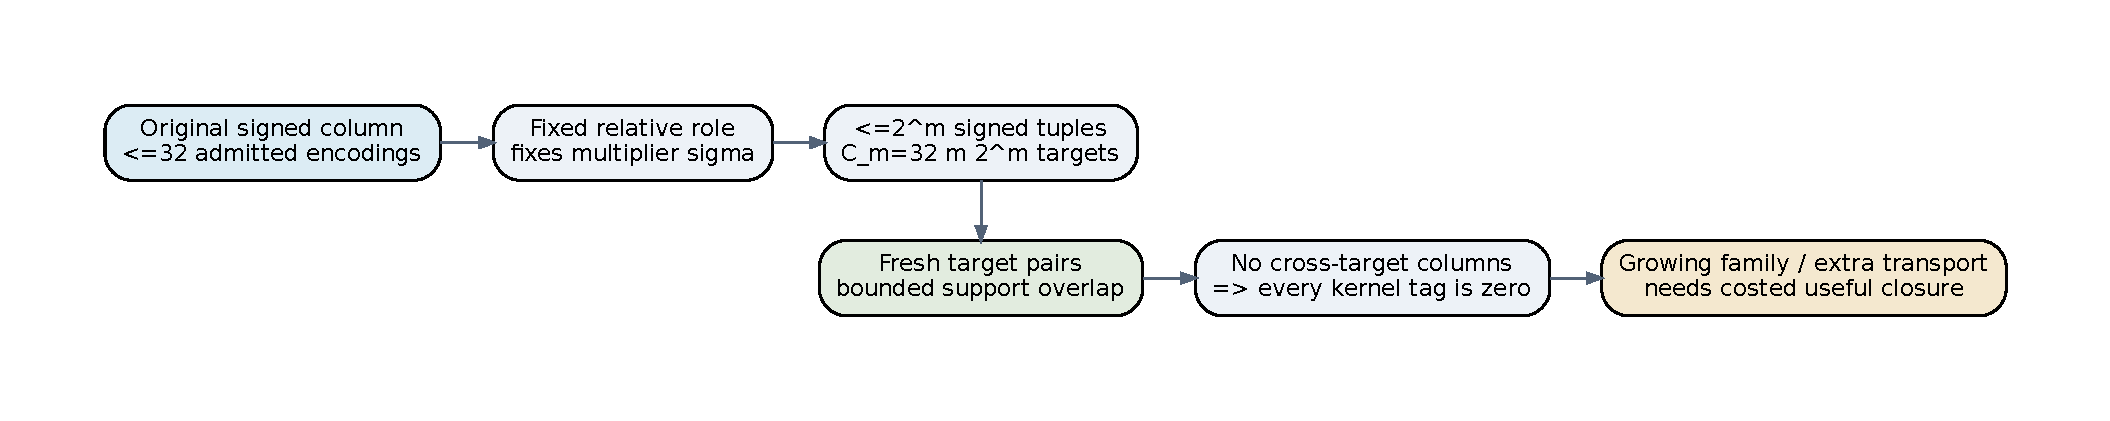
\includegraphics[width=\linewidth]{flow.pdf}

\textbf{One-row bound.} Let $N=\ell-1$ and let $a$ be the number of known
anchor columns. With one online retained row per iid nonzero query, the
previous support has size at most $m(i-1)+a$. Conditional on the history,
the next target can overlap only in a union of that many incidence fibres.
Thus useful tagged-kernel recovery has probability at most
\[
 \frac{C_m}{N}\left(\frac{mt(t-1)}2+at\right).
\]
For $m=2,a=2$, this is $256t(t+1)/N$. Committing to one row online is
essential; selecting from every stored root afterwards uses the next page's
bound. The first overlap is necessary, not sufficient, for recovery.

\scope\quad The original native map/group and sampler refinements remain open.
\newpage
{\Large\bf All roots per target: separated blocks kill the tags}

There are $N/2$ nonzero physical prime-group columns modulo sign. For two
independent uniform nonidentity targets $U,V$, including equal outcomes,
\[
 \Pr[S(U)\cap S(V)\ne\varnothing]
 \le \frac{\sum_P d(P)^2}{N^2}\le\frac{C_m^2}{2N}.
\]
The first inequality is a union of the Cartesian squares of column fibres.
It requires no bound on roots per individual target and no random-support
heuristic. For $t$ such queries, the probability of any cross-query sharing
or anchor hit is at most
\[
 \boxed{\ \frac{C_m^2t(t-1)}{4N}+\frac{aC_mt}{N}\ }.\tag{ALL}
\]
Bounds above $1$ are simply uninformative. Correlated queries such as $T,-T$
do not meet the independence contract.

\textbf{Why this is a recovery obstruction.} Fix one DLP $Q=xG$ and tags
$T_i=a_iG+b_iQ$. Normalize every row of query $i$ to target $T_i$. With no
cross-query sharing or anchor hit, each used column belongs to one block.
For a left-kernel vector $v$, restricting column equations to block $i$ and
evaluating at their hidden logs gives
\[
 \left(\sum_{r\text{ in block }i}v_r\right)T_i=0.
\]
Nonzero $T_i$ has order $\ell$, so each block coefficient sum is zero.
Consequently $v^Ta=v^Tb=0$ for every kernel vector. This permits any number
of rows per query. Hidden logs occur only in the proof, not in oracle inputs.
Additional known logarithm transports change the model.

\textbf{Zero targets and private labels.} Fresh uniform $a,b\in\mathbb F_\ell$
give uniform $T$. Conditional on $T$, $b$ remains uniform since
$a=\log_G(T)-xb$ is unique. However $T=0,b\ne0$ directly reveals $x$;
rejection must not hide it. Among at most $n$ raw label draws, add $n/\ell$
to (ALL) with $t=n$. Failed/no-root draws are charged too. Conditioning a
record on successful decompositions requires a separate selection analysis.

\textbf{Formal owner floor.} \href{https://github.com/aburan28/crypto-lean/pull/39}{crypto-lean PR39}
contains four reusable laws under explicit finite-set or field-matrix
hypotheses. The focused maintained gate passes four named theorems, no
failures and no trusted-native proofs; only standard axioms occur.
\begin{center}\small
\begin{tabular}{lp{3.6in}}
\toprule
Law & Formal conclusion and boundary\\\midrule
\texttt{covered\_card\_le} & Finite union cardinality; degree supplied.\\
\texttt{sharing\_pairs\_card\_le} & Ordered shared-target pairs; diagonals included.\\
\texttt{block\_projection\_image} & Owner-masked field valuation; row semantics supplied.\\
\texttt{separated\_block\_kernel\_tags} & Kernel kills block tags; nonzero targets essential.\\\bottomrule
\end{tabular}\end{center}
Three examples check satisfiable contracts and the zero-target boundary.
The curve/cofactor/map incidence instance, probability bridge and costs are
not supplied by those generic laws. Lean4.35.0 and Mathlib cfc55fc5 stay pinned.
\scope
\newpage
{\Large\bf Constructive successor: pay for useful closure}

\textbf{Growing family gate.} A predeclared family of $D$ templates replaces
$C_m$ by $C_mD$ in ONE. If $D=\ell^\delta$, a future method with actual tight
query cost $\Theta(D^\alpha)$ and an attained useful-collision scale would
have optimistic query exponent
\[
 \frac12+\delta\left(\alpha-\frac12\right).
\]
Thus $\alpha<1/2$ is a prospective target within that model, not sufficient.
A mere upper bound $O(D^\alpha)$ with $\alpha\ge1/2$ cannot disprove another
method. ALL instead has a $D^2$ overlap bound; explicitly returning $D$
witnesses can itself cost $\Omega(D)$. Do not mix these models.

\textbf{Avoid the ratio scan for one supplied column.} Given target $T$ and
one old signed column $P$, form $U=T-P$. Enumerate original inverse
encodings of $P$ and $U$, at most $32$ each, and test ratios $r=w/z$ against
the allowed family. The template $(1,r)$ with multiplier $z$ covers every
admitted witness using that signed column, in at most $1024$ encoding pairs.
Both signs cost at most $2048$ pairs. Identity, chart, raw-distinctness,
original range and cofactor-sum checks remain mandatory.

For a norm-power family $r^q=\omega$, one candidate's membership can be
tested by binary powering without enumerating the family. This is a written
reduction, not a new qualified implementation. Actual original parameters
remain required; a $q=1$ replacement would not test them.

\textbf{The missing search is useful closure.} Choosing the old column is
not free. If every row attaches only one new column to one old column,
singleton peeling removes the tree and no useful kernel remains. For $L$
old physical columns, signed sums of two old columns, including doubles,
give at most $2L^2$ public targets before ratio guards. A fresh target's
closure probability is therefore at most $2L^2/(\ell-1)$.

An optimistic $L\sim t$ closure model suggests $t\sim\ell^{1/3}$, but an
$O(L)$ scan/query then costs order $\ell^{2/3}$. With actually tight query
cost $\Theta(L^\beta)$ at that optimistic scale, the phase exponent would be
$(1+\beta)/3$; beating $1/2$ would require $\beta<1/2$. Neither the scale nor
the useful coefficient is established. A structured implicit selector must
return an original witness with charged setup, growth, lifting, indexing,
memory, kernel and final scalar replay costs.

\textbf{Next discriminator.} Freeze a new anchored-inversion interface with
public target, supplied old column and explicit ratio-family specification.
Then distinguish tree growth from two-old-column closure, retain private tags,
and price the column-selection policy. Target an implicit intersection with
$T-S$; supplied roots, an $L^2$ sum table or an $O(L)$ scan do not meet the
prospective sub-square-root query gate. No such run is scheduled here.

\textbf{Sources and boundaries.} Diem's
\href{https://arxiv.org/pdf/math/0606607}{double-large-prime analysis},
sections2--3, supplies classical graph/recovery context and assumes genus
at least2. His \href{https://doi.org/10.1112/S0010437X10005075}{elliptic extension-field paper},
Proposition2.12, supplies the private-label condition. Shoup's
\href{https://www.shoup.net/papers/dlbounds1.pdf}{generic encoding model}
does not include the coordinate oracle. KB retrieval was unavailable;
novelty is unestablished. No measured exponent or full-base solve is reported.
\scope
\end{document}
